\section{Phase 1 – Selecting Suitable Emotion Recognition Models}\label{sec:experiment-phase1}

After conducting a literature review as discussed in Sections~\ref{sec:fer} and~\ref{sec:ser}, the next task involved identifying and setting up suitable pre-trained models for emotion recognition. The experimental flow is illustrated in Figure~\ref{fig:phase1}. 

\begin{figure*}[h]
    \centering
    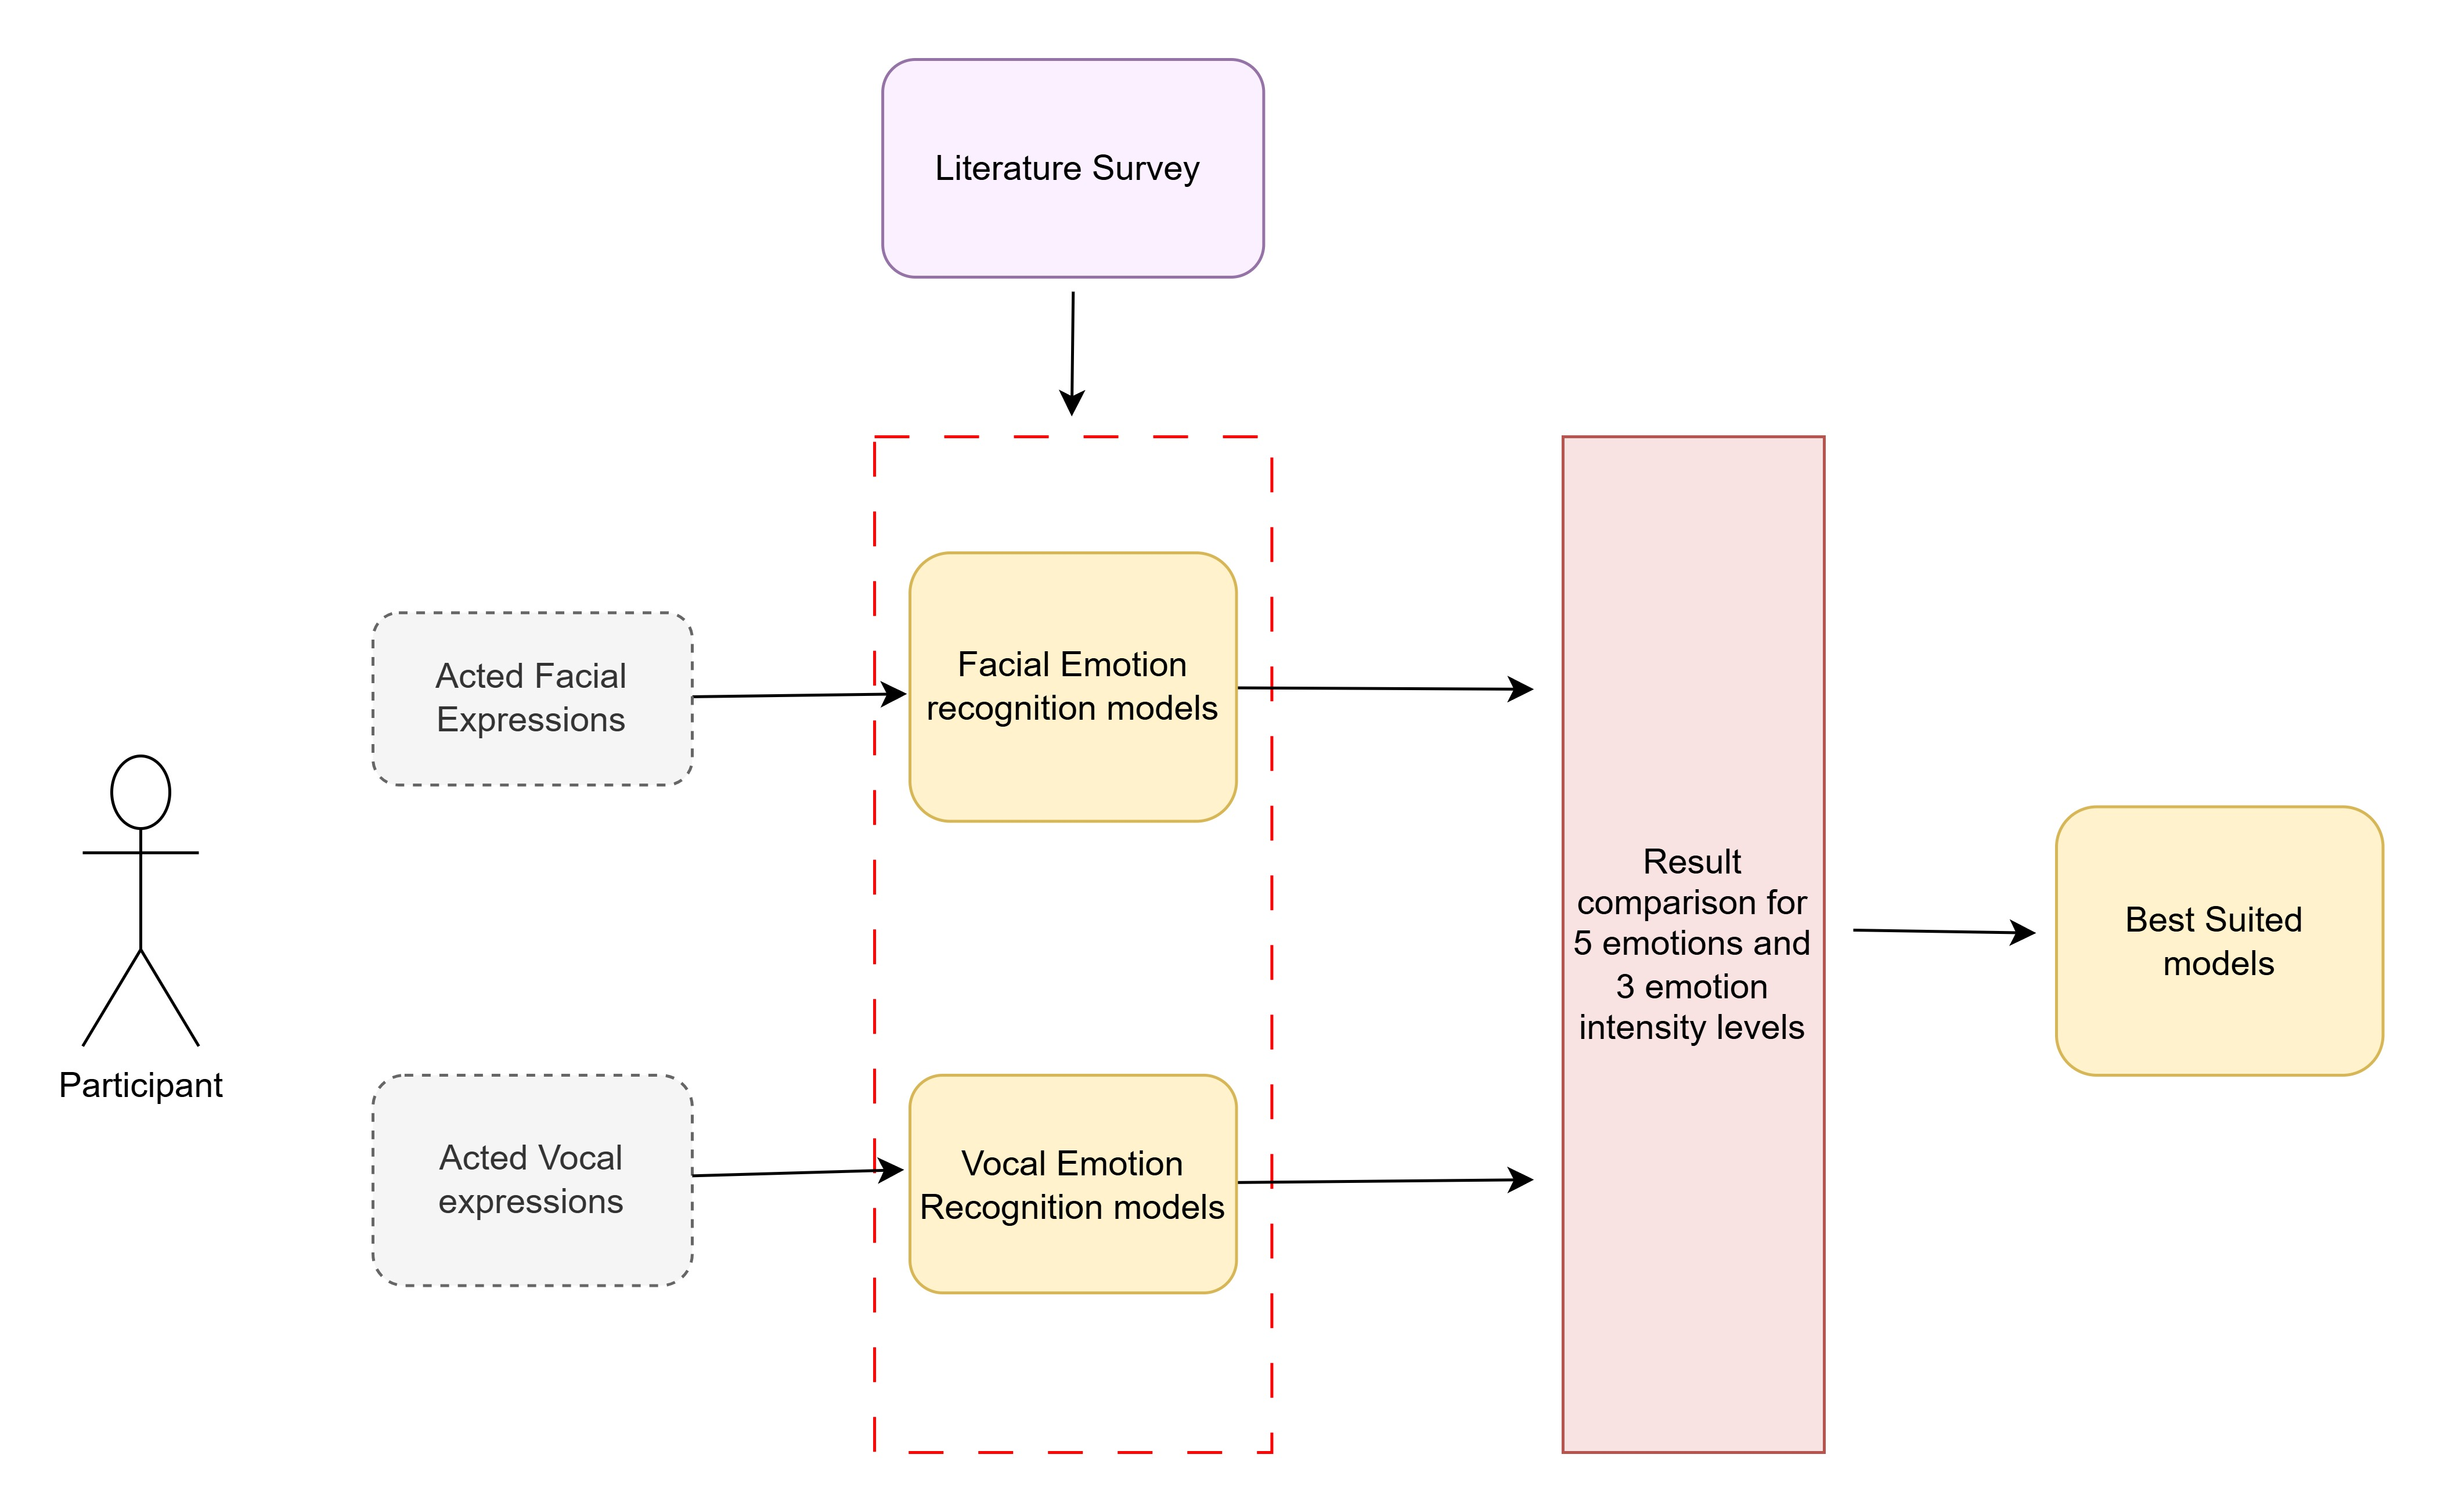
\includegraphics[width=1\textwidth]{img/chapter_03/Phase1.jpg}
    \captionof{figure}{Experimental flow of Phase 1}
    \label{fig:phase1}
\end{figure*}

We initially explored the EmoNet model~\citep{toisoul2021estimation}, available at \url{https://github.com/face-analysis/emonet}, which is well-regarded for arousal-valence detection. However, it presented several technical challenges due to its outdated dependencies, as it was developed in 2021. Although We was able to configure the environment, the model took over four seconds to process a single frame on a CPU, making it unsuitable for real-time applications.

To overcome these issues, We explored alternative options and identified the CAGE expression inference model~\citep{wagner2024cage}, which is optimized for real-time arousal-valence detection. 

Additionally, We found Hume AI’s expression recognition API to be valuable for practical applications. Hume provides real-time facial expression predictions through WebSocket-based streaming, allowing continuous data flow without overloading local resources. It supports a variety of media formats and offers both REST and WebSocket endpoints for batch and live processing, respectively. This makes it a strong candidate for integration with interactive applications.

Based on model performance, practicality, and ease of integration, We selected the CAGE model and the Hume facial expression model for experimental evaluation.

For discrete emotion classification in speech, several datasets are widely available, including RAVDESS~\citep{livingstone2018ryerson}, Emo-DB, and MSP-IMPROV. However, for continuous speech emotion assessment with arousal-valence labeling in English, only a few datasets meet the criteria, such as OMG Emotion, IEMOCAP~\citep{busso2008iemocap}, and MSP-Podcast~\citep{lotfian2017building}. These datasets provide audio clips labeled with arousal and valence scores, enabling a more granular emotional analysis.

Among the available pre-trained models, we identified the wav2vec2 model~\citep{wagner2023dawn} on Hugging Face, which outputs arousal-valence values from speech signals and showed strong compatibility with the project requirements.

Additionally, Hume.ai’s speech emotion recognition system, trained on the large-scale HUME-VB dataset, provides high-performance real-time prediction capabilities. The HUME-VB dataset contains over 280,000 vocalizations from 4,000+ participants across five culturally diverse countries, including the USA, China, India, Venezuela, and South Africa, making it a valuable addition for multilingual and cross-cultural emotion recognition scenarios.

For the experiment, we selected both the \textbf{wav2vec2} model and the \textbf{Hume vocal expression model} to assess and compare their performance in recognizing emotional states from speech input.


\subsection{Facial Expression Experiment Setup}

To evaluate the accuracy of the selected facial models (Hume and CAGE), we conducted an experiment using acted facial expressions. Participants were asked to express five emotions, \textbf{Happy, Angry, Sad, Boredom, and Calm} across three intensity levels: \textbf{Low}, \textbf{Medium}, and \textbf{High}. Each emotion was performed intentionally, and recordings were captured under similar lighting conditions using the webcam. An experiment snapshot is shown in Figure~\ref{fig:facial_expr_experiment}.

\begin{figure*}[h]
    \centering
    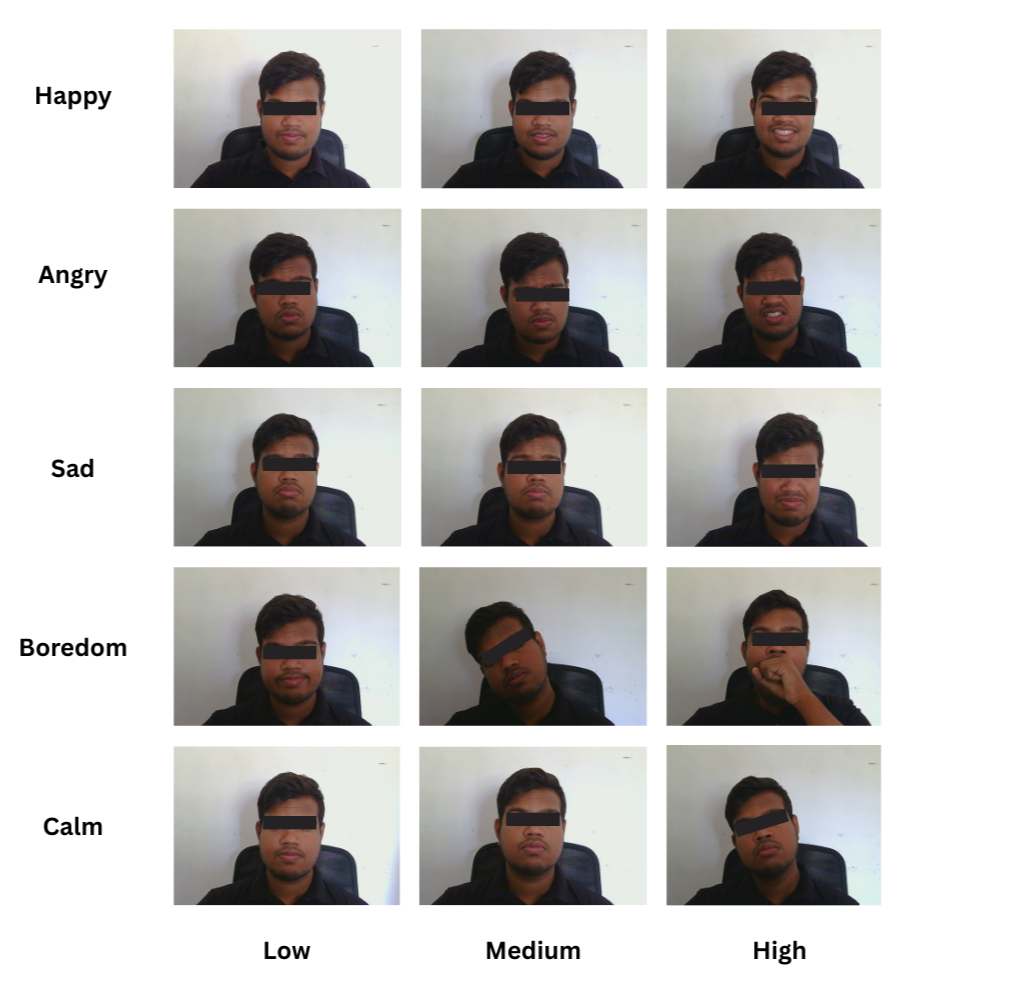
\includegraphics[width=1\textwidth]{img/chapter_03/facial_expr_experiment.png}
    \captionof{figure}{Experiment snapshot for facial expression recognition}
    \label{fig:facial_expr_experiment}
\end{figure*}


\subsection{Vocal Emotion Experiment Setup}

For vocal emotion recognition, participants were asked to read emotion-evoking phrases that are commonly used in scientific emotion corpora such as RAVDESS and IEMOCAP. A total of 15 phrases were used, covering all five target emotions. These phrases were selected to be emotionally neutral in content so that the emotion would be expressed purely through vocal tone and prosody.

\textbf{Emotion phrases used in the experiment:}
\begin{itemize}
    \item \textbf{Happy:} 
    \begin{itemize}
        \item "I’m glad you’re here."
        \item "That was a fantastic surprise."
        \item "You made my day!"
    \end{itemize}
    \item \textbf{Angry:} 
    \begin{itemize}
        \item "This is completely unacceptable."
        \item "I’ve told you this before!"
        \item "Why didn’t you listen to me?"
    \end{itemize}
    \item \textbf{Sad:} 
    \begin{itemize}
        \item "I miss you so much."
        \item "Everything feels so heavy today."
        \item "I just want to be alone."
    \end{itemize}
    \item \textbf{Boredom:} 
    \begin{itemize}
        \item "There’s nothing to do."
        \item "Same thing every day."
        \item "I don’t care anymore."
    \end{itemize}
    \item \textbf{Calm:} 
    \begin{itemize}
        \item "Everything is going to be okay."
        \item "Let’s take a deep breath."
        \item "I’m feeling at peace."
    \end{itemize}
\end{itemize}
